% !Mode:: "TeX:UTF-8"

\BiChapter{深度学习的二分类方法}{}
\label{c:classifer}
中文词语相似度计算本身是一个无监督的回归问题,这增加了解决问题的难度。如果能够将无监督学习转化为有监督学习,并且将回归问题转化为分类问题,就可以利用大量已知的模型,问题解决的难度也将会大大降低。

本章将介绍一种方法,这种方法利用词语在句子中的可替换性计算词语相似度。如果一个“通顺”的句子中的一个词语被替换之后,形成的句子仍然较为“通顺”,则本方法认为原词语和替换的词语较为接近;否则,认为两词语差距较大。本方法从未经处理的生语料库中抽取句子生成数据,并训练一个辅助的二分类器以判定句子的“通顺”与否。二分类器使用深度学习模型构建,以提高模型对整个句子的理解能力。

\BiSection{原理介绍}{}
\label{s:classifer pricinple}
为了更清晰的介绍深度学习的二分类方法,本文将先给出一些形式化的定义。

在深度学习的二分类方法中使用的语料库$\mathcal{C}$是一个句子的多重集合,其中每一个句子是一个词语的序列,即:
\begin{equation}
\mathcal{C} \subset \mathcal{V}^+
\label{e:corpus}
\end{equation}
其中$\mathcal{V}$是所有词语的集合。

替换函数$f_\text{r}$可以将一个句子$s \in \mathcal{C}$中的某个词语$s_i$替换为一个不同的词语$v \ne s_i$,即:
\begin{equation}
f_\text{r}(s, i, v) = (s_1, \dots, s_{i - 1}, v, s_{i + 1}, \dots, s_{|s|})
\end{equation}
对语料库中的句子应用替换函数$f_\text{r}$得到的句子称为替换句:
\begin{equation}
\mathcal{C}_\text{r} = \bigl\{f_\text{r}(s, i, v) \bigm| s \in \mathcal{C}, v \in \mathcal{V}\bigr\}
\end{equation}
一般来说,$\mathcal{C}_\text{r} \cap \mathcal{C} \approx \emptyset$。本课题希望得到一个二分类器$M_\mathcal{C}$,满足:
\begin{equation}
M_\mathcal{C}(s) = 
\begin{cases}
1 & s \in \mathcal{C}, \\
0 & s \in \mathcal{C}_\text{r}
\end{cases}
\end{equation}
使得$M$可以区分原句与替换句。

利用这样的二分类器,我们就可以定义词语对$(v_\text{a}, v_\text{b})$的相似度:
\begin{equation}
\similarity(w_\text{a}, w_\text{b}) = E\Bigl(M_\mathcal{C}\bigl(f_\text{r}(s, i, v_\text{b})\bigr) \Bigm| s \in \mathcal{C}, s_i = v_\text{a}\Bigr)
\end{equation}
其中$E$为数学期望。其中的思想是,利用包含词语$v_\text{a}$的句子以$v_\text{b}$替换得到的替换句测试二分类器$M_\mathcal{C}$,若二分类器容易将这样的替换句误判为原句,则说明词语对$(v_\text{a}, v_\text{b})$相似。为了提高准确性,应同时考虑从$v_\text{a}$到$v_\text{b}$和从$v_\text{b}$到$v_\text{a}$的替换。

\BiSubsection{训练数据生成}{}
为了训练二分类器$M_\mathcal{C}$,我们需要一些带有标注的句子$(x, y) \in \mathcal{V}^+ \times \{0, 1\}$作为训练数据。其中:
\begin{equation}
	y = 
	\begin{cases}
		1 & x \in \mathcal{C}, \\
		0 & x \in \mathcal{C}_\text{r}
	\end{cases}
\end{equation}
原句的生成是非常容易的,只需将$M_\mathcal{C}$中全部的句子标注为$1$即可。而替换句的生成需要一些额外的步骤。

利用随机采样的方法,我们可以生成一些采样句。采样句定义如下:
\begin{equation}
\mathcal{C}_\text{s} = \Bigl\{f_\text{r}(s, i, v) \Bigm| s \in \mathcal{C}, i \sim \mathcal{U}\bigl\{1, |s|\bigr\}, v \sim \mathcal{D}_\mathcal{V}\Bigr\}
\end{equation}
其中$\mathcal{U}$为均匀分布,$\mathcal{D}_\mathcal{V}$为词语在自然语言中出现的概率分布。也就是说,采样句中的被替换词语位置$i$是随机选择的,而替换词语$v$亦是从词语分布中采样得到的。

显然,$\mathcal{C}_\text{s} \subset \mathcal{C}_\text{r}$,而随机采样对于计算机来说是轻而易举的任务。这样,我们就可以通过生成采样句的方式获得用于训练的替换句。

\BiSubsection{循环神经网络}{}
\label{s:classifer rnn}
上文提到,本课题需要训练一个二分类器$M_\mathcal{C}$用于区分原句和替换句。二分类器的输入是一个句子$x \in \mathcal{V}^+$,而输出为$y' = M_\mathcal{C}(x) \in \{0, 1\}$。

循环神经网络(RNN)是一种具有循环连接的神经网络。这类神经网络可以用于进行时间序列的处理,因此常用于自然语言处理领域。

由于各类神经网络均以向量作为输入,因此需要将句子中的词语转化为向量,也就是词嵌入。词嵌入的形式非常简单,设有词嵌入矩阵$E^{|\mathcal{V}| \times n_{\text{embed}}}$,则词嵌入的结果为:
\begin{equation}
e_i = E_{x_i}
\end{equation}
其中$n_{\text{embed}}$是词嵌入维数。由于目前缺少成熟的预训练的中文词嵌入,所以本课题将词嵌入矩阵$E$作为可训练参数,与网络参数同时接受优化算法的优化。

循环神经网络的结构如图\ref{f:rnn}所示。其中,$e_i$如上文所述,作为循环神经网络的输入,而$h_i$是循环神经网络的输出。

\begin{figure}[h]
	\centering
	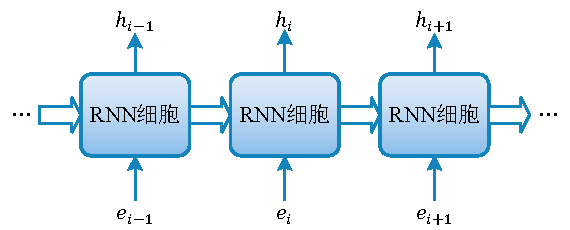
\includegraphics{RNN}
	\caption{RNN结构}
	\label{f:rnn}
	\vspace{-1em}
\end{figure}

RNN细胞可以看作是一个带有可训练参数的函数,每个RNN细胞的可训练参数共享。相邻的RNN细胞之间会传递一些信息,信息的内容取决于RNN细胞的种类。

\BiSubsection{LSTM}{}
\label{s:classifer lstm}
现代的循环神经网络具有多种变种,其中非常著名的一种即是\cite{Hochreiter1997}中提出的LSTM(Long short-term memory)。其经过了\cite{Gers2000}改进,形成了现在常见的LSTM形式。本课题中即采用上述LSTM模型构建二分类器。

LSTM与其它RNN的不同之处在于其独特的细胞结构,如图\ref{f:lstm}所示。LSTM的最大特点是其优秀的“记忆能力”,即能处理时间序列中间隔很长的序列。这得益于LSTM中加入的遗忘门、输入门和逻辑门的设计。

\begin{figure}[h]
	\centering
	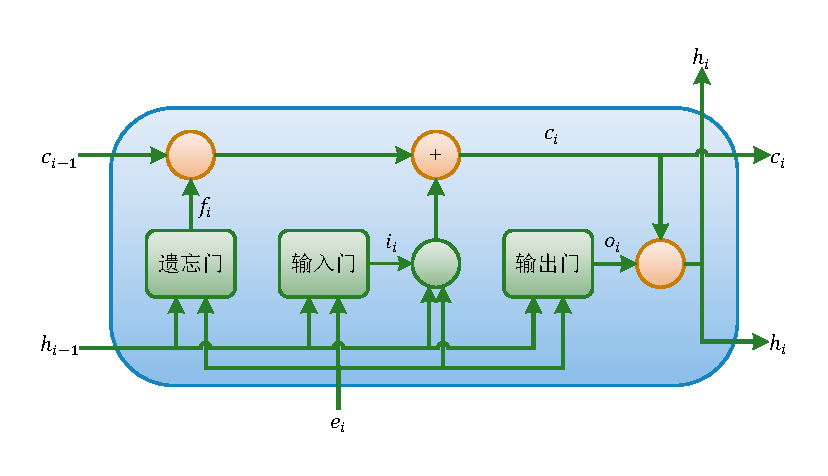
\includegraphics{LSTM}
	\caption{LSTM细胞结构}
	\label{f:lstm}
	\vspace{-1em}
\end{figure}

图\ref{f:lstm}中的$c_i$是LSTM细胞间的隐藏状态,$f_i$为遗忘门,$i_i$为输入门,$o_i$为输出门。公式\ref{e:lstm begin} -- \ref{e:lstm end}给出了一个LSTM细胞的完整定义,其中$W$、$U$、$b$都是可训练参数,而$\sigma$是sigmoid函数,$\circ$是逐项乘积。

\begin{align}
f_i &= \sigma(W_\text{f} e_i + U_\text{f} h_{i - 1} + b_\text{f}) \label{e:lstm begin} \\
i_i &= \sigma(W_\text{i} e_i + U_\text{i} h_{i - 1} + b_\text{i}) \\
o_i &= \sigma(W_\text{o} e_i + U_\text{o} h_{i - 1} + b_\text{o}) \\
c_i &= f_i \circ c_{i - 1} + i_i \circ \tanh(W_\text{c} e_i + U_\text{c} h_{i - 1} + b_\text{c}) \\
h_i &= o_i \circ \tanh(c_i) \label{e:lstm end}
\end{align}

\BiSubsection{深层LSTM}{}
与其它深度学习模型类似,LSTM网络也可以增加模型的层数以加强模型的学习能力。文献\cite{Sak2014}中给出了多种LSTM与RNN层叠加的方案。本课题使用两个LSTM层叠加的方式,使一个LSTM层的输出向量作为另一个LSTM层的输入向量,如图\ref{f:deep lstm}所示。

\begin{figure}[h]
	\centering
	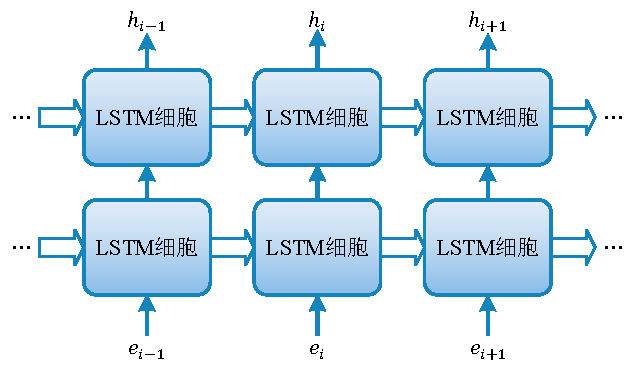
\includegraphics{deep-LSTM}
	\caption{深层LSTM}
	\label{f:deep lstm}
	\vspace{-1em}
\end{figure}

\BiSubsection{分类结果生成}{}
LSTM网络的输出向量最终需要转换为一个二元的输出$y' \in \{0, 1\}$,考虑到使用连续变量能够更容易进行运算,本课题使$y' \in [0, 1]$。

本课题中使用逻辑回归来完成上面的任务。逻辑回归函数如公式\ref{e:logit}所示:
\begin{equation}
F(x) = \frac{1}{1 + e^{-(\beta_0 + \beta_1 x)}}
\label{e:logit}
\end{equation}
其中$\beta_0$与$\beta_1$都是可训练参数。本课题取LSTM网络的最后一个输出为整个网络的输出向量,并应用逻辑回归函数得到分类结果。即:
\begin{equation}
y' = F(h_{|s|})
\end{equation}

为了提高模型性能,本课题还尝试在LSTM输出后增加一个全连接层。此时输出的二分类结果如下:
\begin{equation}
y' = F\bigl(\sigma(W_\text{full} h_{|s|} + b_\text{full})\bigr)
\end{equation}

\BiSubsection{模型训练}{}
\label{s:classifer p-training}
为了训练一个深度学习,需要定义一个损失函数,并且使用一种优化方法来最小化损失函数的值。

损失函数是一种用于衡量预测值$y'$与真实值$y$之间的偏差的函数。当$y' = y$时,$L(y', y) = 0$;而当$y' \neq y$时,$L(y', y) > 0$。一般而言,预测值与真实值之间的偏差越大,损失函数的值也应越大。这样使用数值优化的方法来最小化损失函数的值,就可以得到预测更为真实的模型。

在损失函数的选择方面,本课题选择了二分类问题常用的对数损失函数。对数损失函数的形式如下:
\begin{equation}
L(y', y) = -\bigl(y \log(y') + (1 - y) \log(1 - y')\bigr)
\end{equation}

由于采样句的数量可能与原句不相等,因此会形成不平衡数据集。为了将数据集平衡化,在汇总训练数据的损失函数值时应为每个训练数据赋予一个权重$y(k - 1) + 1$。其中,$k$是训练集中采样居与原句的比例。这样,原句和采样句在训练中占有的权重就是相等的了。最终汇总的损失函数值如下:
\begin{equation}
\sum\bigl(y(k - 1) + 1\bigr) L(y', y)
\end{equation}

深度学习模型的训练大多使用基于梯度下降的优化算法。传统的随机梯度下降方法需要人为指定一个学习速率,并且在训练中途还可能需要进行学习速率的调整,这会给实验带来更多的麻烦。而一些自适应学习速率的优化算法则可以在学习过程中自行调节学习速率,例如Adagrad\citeup{Duchi2011}、Adadelta\citeup{Zeiler2012}、RMSprop\footnote{RMSprop并不是一个在论文中发表的算法,它是在多伦多大学的一个课堂讲义(\url{http://www.cs.toronto.edu/~tijmen/csc321/slides/lecture_slides_lec6.pdf})中被提出的。}与Adam\citeup{Kingma2014}。为了降低实验的复杂程度,本课题使用了\cite{Ruder2016}中推荐的Adam算法进行模型训练。

\BiSection{程序实现}{}
\label{s:classifer implementation}
为了完成深度学习的二分类方法,本项目实现了一个可以处理原始语料、构建模型并进行训练的系统,其结构如图\ref{f:classfier overall}所示。
\begin{figure}[h]
	\centering
	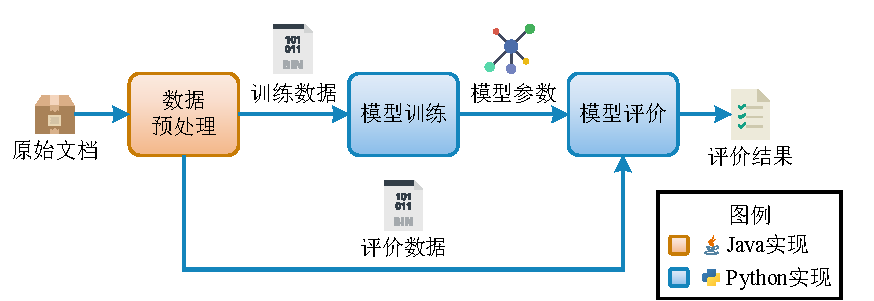
\includegraphics{Cl-overall}
	\caption{整体结构}
	\label{f:classfier overall}
	\vspace{-1em}
\end{figure}

程序实现分为数据预处理、模型训练和模型评价三个模块,根据模块特点的不同,分别使用了Java和Python两种编程语言实现。

\BiSubsection{数据预处理}{}
\label{s:classfier preprocess}
由于Python的文本处理性能较差,会花费过长的时间,数据预处理的程序使用Java语言编写。预处理程序的结构如图\ref{f:classfier preprocess}所示。

\begin{figure}[h]
	\centering
	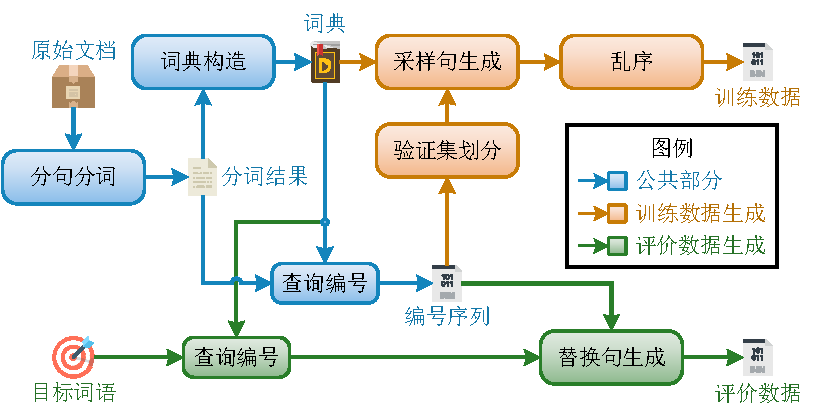
\includegraphics{Cl-preprocess}
	\caption{数据预处理}
	\label{f:classfier preprocess}
	\vspace{-1em}
\end{figure}

本课题使用了清华大学THUCTC工具包中提供的THUCNews数据集作为语料库。该语料库中的内容为从新浪新闻中得到的新闻文档,属于无标注的生语料库,以文本形式存储在文件中。

为了提高模型的准确度,本课题的深度学习模型没有采用一些早期深度学习工作中常用的直接将文档切分为固定长度序列的方式,而是以句为单位进行训练。句子的识别只需要根据简单的标点符号规则,本课题最初实现的句子分割器与后来使用的LTP平台均是如此实现。

接下来对句子进行分词和词性标注。本课题尝试了多种现有的分词工具,包括Java语言的Ansj,ltp4j与Python语言的结巴分词。经过对比分词工具对测试集中词语的切分准确度,最终确定使用Ansj的NLP分词模式。由于部分分词工具的运行速度十分缓慢,分词和词性标注的结果以序列化的方式存储在磁盘上,以备后续步骤使用。

分词和词性标注的结果会被程序读取两次。第一次读取的目的是构造词典,由于词汇量过大,会对词嵌入步骤带来严重的麻烦,本课题将词典中词语的数量限制在500000个,超出词典大小的词语以它们的词性来代替。为了方便词嵌入,词典中的每个词语均赋予一个整数编号。第二次读取数据则是为了将词语序列转换为编号序列,以备后续步骤使用。

生成的序号序列会按照比例随机划分为训练集和验证集。训练集和验证集的后续处理步骤相同。

采样过程如上文中采样句的定义所述,会随机挑选被替换词和替换用词进行替换。在实际实验中,每个原句产生了5个采样句。

为了使学习的结果更加稳定,上述步骤得到的结果最终会被乱序处理。由于数据量过大,乱序处理无法在内存中进行。因此本课题使用了外存储器辅助完成乱序,如算法\ref{a:shuffling}所述。

\begin{algorithm}[h]
	\KwData{待乱序序列$X$}
	\KwResult{乱序后序列$Y$}
	\For{$i$ in $[1, n_\text{split}]$}{
		以写入模式打开临时文件$F_i$\;
	}
	\For{$x$ in $X$}{
		设$i$为$1$ -- $n_\text{split}$之间的随机数\;
		将$x$写入$F_i$\;
	}
	\For{$i$ in $[1, n_\text{split}]$}{
		以读取模式重新打开$F_i$\;
		从$F_i$中读取全部内容$Y_\text{split}$\;
		在$Y_\text{split}$上执行内存乱序算法\;
		\For{$y$ in $Y_\text{split}$}{
			输出$y$\;
		}
	}
	\caption{外存储器乱序算法}
	\label{a:shuffling}
\end{algorithm}

为了方便基于TensorFlow框架的Python程序读取数据,数据预处理阶段使用TFRecords格式保存数据。这样就可以避免书写Python程序读取数据,而通过TensorFlow中定义的reader来完成,避免数据的读取成为速度瓶颈。

\BiSubsection{模型训练}{}
\label{s:classifer training}
模型训练使用了Python语言的TensorFlow框架。该框架既可以通过简洁的API直接生成神经网络层,也可以使用底层的矩阵操作对数据进行细致的调整。在运行时,TensorFlow框架运用了CUDA技术,可以充分利用计算机的GPU资源。

为了平衡训练的速度和稳定性,各类基于梯度下降的学习算法往往需要将数据划分为mini-batch,而每一个mini-batch的数据在TensorFlow平台中由一个多维数组来表述。这意味着在生成mini-batch时,需要将变长序列填补成固定长度的序列。利用TensorFlow框架提供的队列机制可以完成这一任务,它可以在取出内容时动态填补序列。每个序列需要一个单独的线程进行驱动,这将在后文中讲解。

在利用TensorFlow框架进行开发时,首先应进行数据的读取。由于数据预处理程序已经将数据输出为TFRecords格式,这里可以使用reader轻松地读取数据。

接下来应构建TensorFlow图。TensorFlow图由一系列的操作组成。每个操作接受一定数量(也可能没有)的Tensor作为输入,并且产生一个Tensor作为输出。TensorFlow框架提供了包括Tensor变形、数学运算、神经网络层等API来应用操作。根据第\ref{s:classifer pricinple}节中所列出的表达式,就可以构造出完整的TensorFlow图。在构造过程中,应该注意设置设备布局,将适合CPU计算的操作布局在CPU上布局,而将适合GPU计算的操作在GPU上布局。

为了简化程序的编写,TensorFlow框架提供了Supervisor机制以管理训练过程。Supervisor负责产生驱动队列的线程,保存模型参数,并TensorBoard数据。创建Supervisor后,程序根据当前训练步数决定运行训练数据或验证数据。

\BiSubsection{模型评价}{}
为了评价模型,在数据的预处理阶段就需要根据目标词对生成用于评价的替换句。为了编程方便,评价数据的生成与训练数据的生成同时进行,这样很多用于训练数据生成的代码和中间数据都可以复用。程序只需要过滤所有的原句,查找目标词语。如果发现目标词语,则用词语对中对应的词语生成替换句。评价数据的数据格式与训练数据大致相同,只需要将原本的正负例标注换成用于生成替换句的词语对ID。由于评价数据不影响模型训练,因此无需进行乱序操作。

将评价数据输入第\ref{s:classifer training}小节中构建的深度学习模型中,就可以得到每个句子的预测值$y'$,这样,用于TensorFlow图构建的大部分程序可以被复用。根据词语对ID将预测值分组,并且求预测值的平均值,就可以得到每个词语对的相似度评价。对于词典外词汇,由所有句子的预测值平均值代替本词语对的预测值平均值。由于模型性能的评价指标是Spearman等级相关系数,与预测值的绝对值无关。因此无需对输出做任何缩放处理。Spearman等级相关系数的计算由Excel软件完成。

\BiSection{实验结果}{}